% Created 2026-04-23 Thu 23:45
% Intended LaTeX compiler: pdflatex
\documentclass{article}
\usepackage[utf8]{inputenc}
\usepackage[T1]{fontenc}
\usepackage{graphicx}
\usepackage{longtable}
\usepackage{wrapfig}
\usepackage{rotating}
\usepackage[normalem]{ulem}
\usepackage{amsmath}
\usepackage{amssymb}
\usepackage{capt-of}
\usepackage{hyperref}

\usepackage{fancyhdr}
\usepackage[top=25mm, left=25mm, right=25mm]{geometry}
\usepackage{longtable}
\fancyhead[R]{}
\setlength\headheight{43.0pt}
\usepackage{tabularx}
\usepackage{longtable}
\author{Leonardo Rodriguez, Jóse Jacome,Samuel Churaco,}
\date{2026-04-08 Grupo 9}
\title{Taller de Configuracion de Entorno WSL}
\hypersetup{
 pdfauthor={Leonardo Rodriguez, Jóse Jacome,Samuel Churaco,},
 pdftitle={Taller de Configuracion de Entorno WSL},
 pdfkeywords={},
 pdfsubject={},
 pdfcreator={Emacs 27.1 (Org mode 9.7.5)}, 
 pdflang={Espanol}}
\begin{document}

\maketitle
\fancyhead[C]{
\includegraphics[scale=0.05]{../images/logoEPN.jpg}\\
orESCUELA POLITECNICA NACIONAL\\FACULTAD DE INGENIERIA DE SISTEMAS\\
ARQUITECTURA DE COMPUTADORES}
\thispagestyle{fancy}

\section{Objetivos}
\label{sec:orge959553}

\begin{itemize}
\item Configurar y validar el entorno de trabajo para la asignatura de Arquitectura de Computadores en Linux o WSL.
\item Verificar la instalacion de herramientas base: mamba/anaconda (Python), Emacs y \LaTeX.
\item Documentar evidencias tecnicas mediante capturas y comandos ejecutados.
\end{itemize}

\section{Instrucciones}
\label{sec:orgf0dbb9a}

\begin{enumerate}
\item Realice todas las actividades en Linux o en WSL.
\item En cada sección ejecute los comandos solicitados y registre la salida en el bloque correspondiente.
\item Guarde el archivo y exporte a pdf con el comando `org-latex-export-to-pdf`.
\item Verifique que estén todos los nombres de los integrantes del grupo
de trabajo. Los grupos para este trabajo están en \href{https://epnecuador.sharepoint.com/:x:/s/ICCD332-ArquitecturaComputadores/IQCjNuELSDbJTb42EfrLL2ksATBSbitbZ9\_iFLJxIiCtSr0?e=gowv5I}{Equipos de Trabajo}.
\item Verifique que en las distintas secciones de este archivo esté
identificado con nombre e email el aporte del estudiante.
\end{enumerate}

Si require insertar una imagen, crear una carpeta \texttt{images} y colocar
la imagen dentro. Para llamar la imagen desde Emacs use \texttt{C-c C-l} y
busque el archivo o escriba:Puede insertar una imagen con la sintaxis:

\begin{verbatim}
[[./images/image1.jpg]]
\end{verbatim}
\section{Actividades}
\label{sec:org8276738}
\subsection{Configuración de WSL con Ubuntu, \LaTeX, Python e Emacs}
\label{sec:org5398d07}

\begin{enumerate}
\item Verificacion de entorno mamba/anaconda

-Leonardo Rodriguez
\begin{verbatim}
   mamba info
\end{verbatim}

\begin{verbatim}

	  libmamba version : 2.5.0
	     mamba version : 2.5.0
	      curl version : libcurl/8.19.0 OpenSSL/3.6.1 zlib/1.3.2 zstd/1.5.7 libssh2/1.11.1 nghttp2/1.68.1 mit-krb5/1.22.2
	libarchive version : libarchive 3.8.6 zlib/1.3.2 liblzma/5.8.2 bz2lib/1.0.8 liblz4/1.10.0 libzstd/1.5.7 liblzo2/2.10 openssl/3.5.5 libb2/bundled
	  envs directories : /home/josejacome_epn/.local/share/mamba/envs
	     package cache : /home/josejacome_epn/.local/share/mamba/pkgs
			     /home/josejacome_epn/.mamba/pkgs
	       environment : iccd332 (active)
	      env location : /home/josejacome_epn/.local/share/mamba/envs/iccd332
	 user config files : /home/josejacome_epn/.mambarc
    populated config files : 
	  virtual packages : __unix=0=0
			     __linux=6.6.87=0
			     __glibc=2.39=0
			     __archspec=1=x86_64_v3
			     __cuda=13.2=0
		  channels : https://conda.anaconda.org/conda-forge/linux-64
			     https://conda.anaconda.org/conda-forge/noarch
	  base environment : /home/josejacome_epn/.local/share/mamba
		  platform : linux-64
\end{verbatim}

-José Jácome
\begin{verbatim}
   mamba info
\end{verbatim}

\begin{verbatim}

	  libmamba version : 2.5.0
	     mamba version : 2.5.0
	      curl version : libcurl/8.19.0 OpenSSL/3.6.1 zlib/1.3.2 zstd/1.5.7 libssh2/1.11.1 nghttp2/1.68.1 mit-krb5/1.22.2
	libarchive version : libarchive 3.8.6 zlib/1.3.2 liblzma/5.8.2 bz2lib/1.0.8 liblz4/1.10.0 libzstd/1.5.7 liblzo2/2.10 openssl/3.5.5 libb2/bundled
	  envs directories : /home/josejacome_epn/.local/share/mamba/envs
	     package cache : /home/josejacome_epn/.local/share/mamba/pkgs
			     /home/josejacome_epn/.mamba/pkgs
	       environment : iccd332 (active)
	      env location : /home/josejacome_epn/.local/share/mamba/envs/iccd332
	 user config files : /home/josejacome_epn/.mambarc
    populated config files : 
	  virtual packages : __unix=0=0
			     __linux=6.6.87=0
			     __glibc=2.39=0
			     __archspec=1=x86_64_v3
			     __cuda=13.2=0
		  channels : https://conda.anaconda.org/conda-forge/linux-64
			     https://conda.anaconda.org/conda-forge/noarch
	  base environment : /home/josejacome_epn/.local/share/mamba
		  platform : linux-64
\end{verbatim}

-Samuel Churaco
\begin{verbatim}
   mamba info
\end{verbatim}

\begin{verbatim}

	  libmamba version : 2.5.0
	     mamba version : 2.5.0
	      curl version : libcurl/8.19.0 OpenSSL/3.6.1 zlib/1.3.2 zstd/1.5.7 libssh2/1.11.1 nghttp2/1.68.1 mit-krb5/1.22.2
	libarchive version : libarchive 3.8.6 zlib/1.3.2 liblzma/5.8.2 bz2lib/1.0.8 liblz4/1.10.0 libzstd/1.5.7 liblzo2/2.10 openssl/3.5.5 libb2/bundled
	  envs directories : /home/josejacome_epn/.local/share/mamba/envs
	     package cache : /home/josejacome_epn/.local/share/mamba/pkgs
			     /home/josejacome_epn/.mamba/pkgs
	       environment : iccd332 (active)
	      env location : /home/josejacome_epn/.local/share/mamba/envs/iccd332
	 user config files : /home/josejacome_epn/.mambarc
    populated config files : 
	  virtual packages : __unix=0=0
			     __linux=6.6.87=0
			     __glibc=2.39=0
			     __archspec=1=x86_64_v3
			     __cuda=13.2=0
		  channels : https://conda.anaconda.org/conda-forge/linux-64
			     https://conda.anaconda.org/conda-forge/noarch
	  base environment : /home/josejacome_epn/.local/share/mamba
		  platform : linux-64
\end{verbatim}

\item Verificacion de Python

\begin{itemize}
\item Leonardo Rodriguez
\end{itemize}
\begin{verbatim}
   python --version
\end{verbatim}

\begin{verbatim}
Python 3.11.15
\end{verbatim}


-José Jácome
\begin{verbatim}
   python --version
\end{verbatim}

\begin{verbatim}
Python 3.11.15
\end{verbatim}


-Samuel Churaco
\begin{verbatim}
   python --version
\end{verbatim}

\begin{verbatim}
Python 3.11.15
\end{verbatim}

\item Verificacion de Emacs

-Leonardo Rodriguez
\begin{verbatim}
   emacs --version
\end{verbatim}

\begin{verbatim}
GNU Emacs 29.3
Copyright (C) 2024 Free Software Foundation, Inc.
GNU Emacs comes with ABSOLUTELY NO WARRANTY.
You may redistribute copies of GNU Emacs
under the terms of the GNU General Public License.
For more information about these matters, see the file named COPYING.
\end{verbatim}
\end{enumerate}


\begin{itemize}
\item José Jácome
\end{itemize}
\begin{verbatim}
   emacs --version
\end{verbatim}

\begin{verbatim}
GNU Emacs 29.3
Copyright (C) 2024 Free Software Foundation, Inc.
GNU Emacs comes with ABSOLUTELY NO WARRANTY.
You may redistribute copies of GNU Emacs
under the terms of the GNU General Public License.
For more information about these matters, see the file named COPYING.
\end{verbatim}


-Samuel Churaco
\begin{verbatim}
   emacs --version
\end{verbatim}

\begin{verbatim}
GNU Emacs 29.3
Copyright (C) 2024 Free Software Foundation, Inc.
GNU Emacs comes with ABSOLUTELY NO WARRANTY.
You may redistribute copies of GNU Emacs
under the terms of the GNU General Public License.
For more information about these matters, see the file named COPYING.
\end{verbatim}



\begin{enumerate}
\item Verificacion de \LaTeX{}

-Leonardo Rodriguez
\begin{verbatim}
   latex --version
\end{verbatim}

\begin{verbatim}
   pdfTeX 3.141592653-2.6-1.40.25 (TeX Live 2023/Debian)
   kpathsea version 6.3.5
   Copyright 2023 Han The Thanh (pdfTeX) et al.
   There is NO warranty.  Redistribution of this software is
   covered by the terms of both the pdfTeX copyright and
   the Lesser GNU General Public License.
   For more information about these matters, see the file
   named COPYING and the pdfTeX source.
   Primary author of pdfTeX: Han The Thanh (pdfTeX) et al.
   Compiled with libpng 1.6.43; using libpng 1.6.43
   Compiled with zlib 1.3; using zlib 1.3
   Compiled with xpdf version 4.04
\end{verbatim}

-José Jácome
\begin{verbatim}
   latex --version
\end{verbatim}

\begin{verbatim}
   pdfTeX 3.141592653-2.6-1.40.25 (TeX Live 2023/Debian)
   kpathsea version 6.3.5
   Copyright 2023 Han The Thanh (pdfTeX) et al.
   There is NO warranty.  Redistribution of this software is
   covered by the terms of both the pdfTeX copyright and
   the Lesser GNU General Public License.
   For more information about these matters, see the file
   named COPYING and the pdfTeX source.
   Primary author of pdfTeX: Han The Thanh (pdfTeX) et al.
   Compiled with libpng 1.6.43; using libpng 1.6.43
   Compiled with zlib 1.3; using zlib 1.3
   Compiled with xpdf version 4.04
\end{verbatim}

-Samuel Churaco
\begin{verbatim}
   latex --version
\end{verbatim}

\begin{verbatim}
   pdfTeX 3.141592653-2.6-1.40.25 (TeX Live 2023/Debian)
   kpathsea version 6.3.5
   Copyright 2023 Han The Thanh (pdfTeX) et al.
   There is NO warranty.  Redistribution of this software is
   covered by the terms of both the pdfTeX copyright and
   the Lesser GNU General Public License.
   For more information about these matters, see the file
   named COPYING and the pdfTeX source.
   Primary author of pdfTeX: Han The Thanh (pdfTeX) et al.
   Compiled with libpng 1.6.43; using libpng 1.6.43
   Compiled with zlib 1.3; using zlib 1.3
   Compiled with xpdf version 4.04
\end{verbatim}
\end{enumerate}


\subsection{Comandos Emacs Tutorial}
\label{sec:org7d733f0}

<Leonardo Rodriguez>
\begin{longtable}{|p{0.2\linewidth}|p{0.3\linewidth}|p{0.2\linewidth}|p{0.3\linewidth}|}
\textbf{Comando} & \textbf{Descripción} & \textbf{Comando} & \textbf{Descripción}\\[0pt]
\hline
\endfirsthead
\multicolumn{4}{l}{Continued from previous page} \\[0pt]
\hline

\textbf{Comando} & \textbf{Descripción} & \textbf{Comando} & \textbf{Descripción} \\[0pt]

\hline
\endhead
\hline\multicolumn{4}{r}{Continued on next page} \\
\endfoot
\endlastfoot
\hline
- C-SPC & - Seleccionar todo lo que necesites ya sea copiar o eliminar & - C-w & - Cortar lo que tengas seleccionado\\[0pt]
\hline
- C-/ & - Comando para deshacer todo lo que hayas escrito como un control z tradicional & - C-k & - Eliminar toda una linea\\[0pt]
\hline
- C-s & - Busqueda de pala hacia adelante & - C-r & - Busqueda de palabras hacia atras\\[0pt]
\hline
\end{longtable}

<José Jácome>
\begin{longtable}{|p{0.2\linewidth}|p{0.3\linewidth}|p{0.2\linewidth}|p{0.3\linewidth}|}
\textbf{Comando} & \textbf{Descripción} & \textbf{Comando} & \textbf{Descripción}\\[0pt]
\hline
\endfirsthead
\multicolumn{4}{l}{Continued from previous page} \\[0pt]
\hline

\textbf{Comando} & \textbf{Descripción} & \textbf{Comando} & \textbf{Descripción} \\[0pt]

\hline
\endhead
\hline\multicolumn{4}{r}{Continued on next page} \\
\endfoot
\endlastfoot
\hline
- C-n & - Baja toda una línea en la misma dirección, es como si bajara en NEXT & - C-M-v & - Mueve todo un texto de una ventana a otra sin cambiar la ventana ya activa\\[0pt]
\hline
- C-x C-b & - Muestra todos los buffers activos, como los procesos de emacs & - C-x f & - Cambia el tamaño del margen\\[0pt]
\hline
- C-x u & - Deshace las acciones hechas & - C-g & - Cancela un comando\\[0pt]
\hline
\end{longtable}

<Samuel Churaco>
\begin{longtable}{|p{0.2\linewidth}|p{0.3\linewidth}|p{0.2\linewidth}|p{0.3\linewidth}|}
\textbf{Comando} & \textbf{Descripción} & \textbf{Comando} & \textbf{Descripción}\\[0pt]
\hline
\endfirsthead
\multicolumn{4}{l}{Continued from previous page} \\[0pt]
\hline

\textbf{Comando} & \textbf{Descripción} & \textbf{Comando} & \textbf{Descripción} \\[0pt]

\hline
\endhead
\hline\multicolumn{4}{r}{Continued on next page} \\
\endfoot
\endlastfoot
\hline
- C-h o & - Se puede saltar de ventanas sin el uso del mouse & - C-y & - Pega algo que se copio anteriormente\\[0pt]
\hline
- M-w & - Nos permite copiar algo seleccionado & - C-x 1 & - Nos quedamos con una sola ventana\\[0pt]
\hline
- C-d & - Borra caracteres al inverzo & - C-w & - Corta algo seleccionado\\[0pt]
 &  &  & \\[0pt]
\hline
\end{longtable}


\subsection{Comandos Emacs Juego}
\label{sec:orgb2ea20c}
En la anterior sección usted revisó los comandos de mayor interés
sobre la manipulación de Emacs. Es hora de poner en práctica sus
conocimientos. Realice unas 3 visitas al juego  \href{https://chat.qwen.ai/s/deploy/t\_23ff57ef-b59a-4bd7-9b79-54679b33686d}{Emacs-Trainer} y apunte
en la siguiente tabla su puntaje.

Leonardo Rodriguez:
\begin{center}
\begin{tabular}{rr}
\hline
iteración & Puntaje\\[0pt]
\hline
1 & 128\\[0pt]
2 & 140\\[0pt]
3 & 135\\[0pt]
\hline
\end{tabular}
\end{center}

-Intento 1
\begin{center}
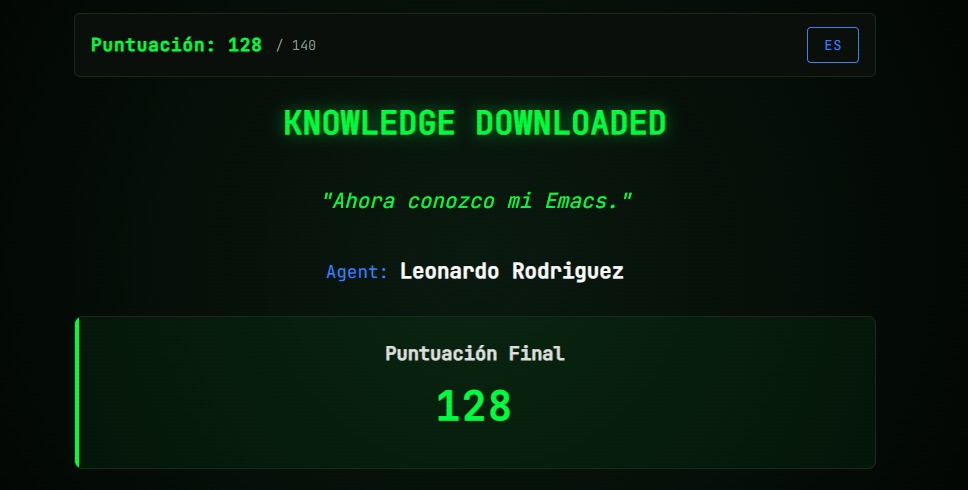
\includegraphics[width=.9\linewidth]{Fotos/Intento1.jpeg}
\end{center} 
-Intento2
\begin{center}
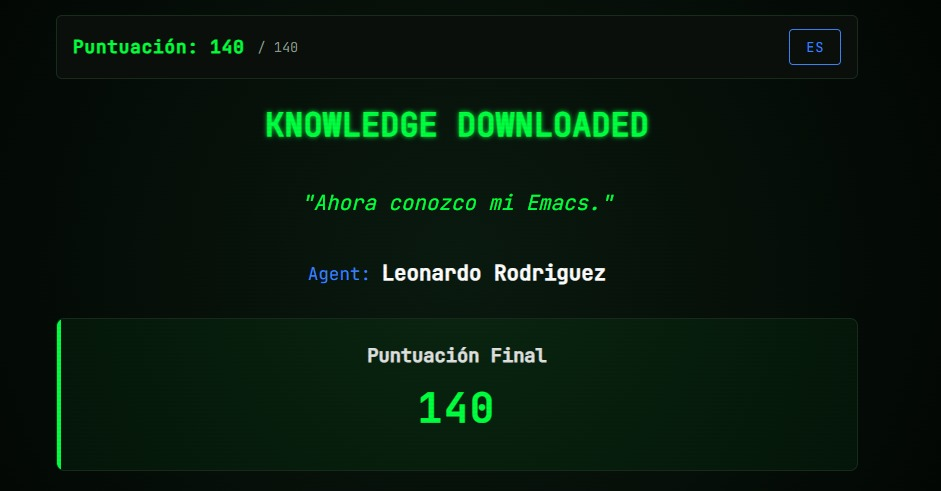
\includegraphics[width=.9\linewidth]{Fotos/Intento2.jpeg}
\end{center}
-Intento3
\begin{center}
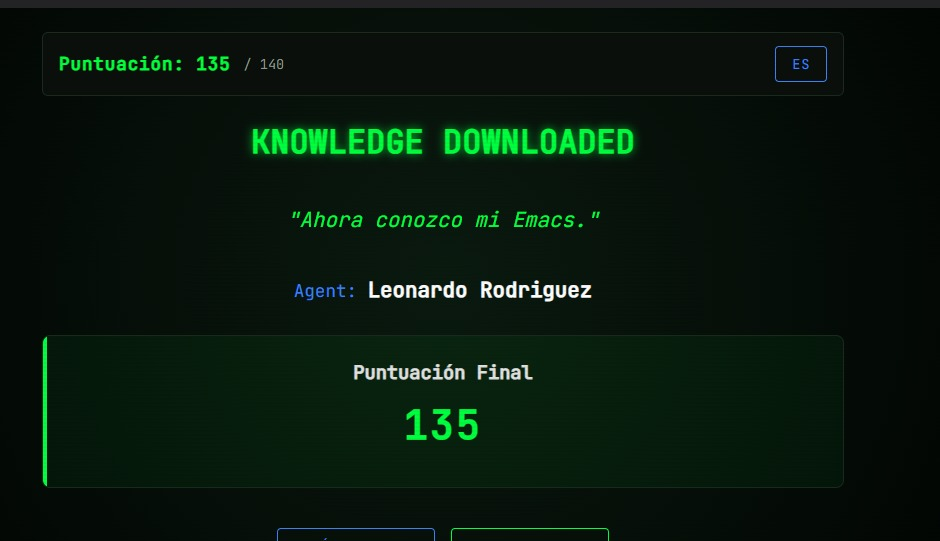
\includegraphics[width=.9\linewidth]{Fotos/Intento3.jpeg}
\end{center}


José Jácome:
\begin{center}
\begin{tabular}{rr}
\hline
iteración & Puntaje\\[0pt]
\hline
1 & 111\\[0pt]
2 & 126\\[0pt]
3 & 130\\[0pt]
\hline
\end{tabular}
\end{center}


-Intento 1
\begin{center}
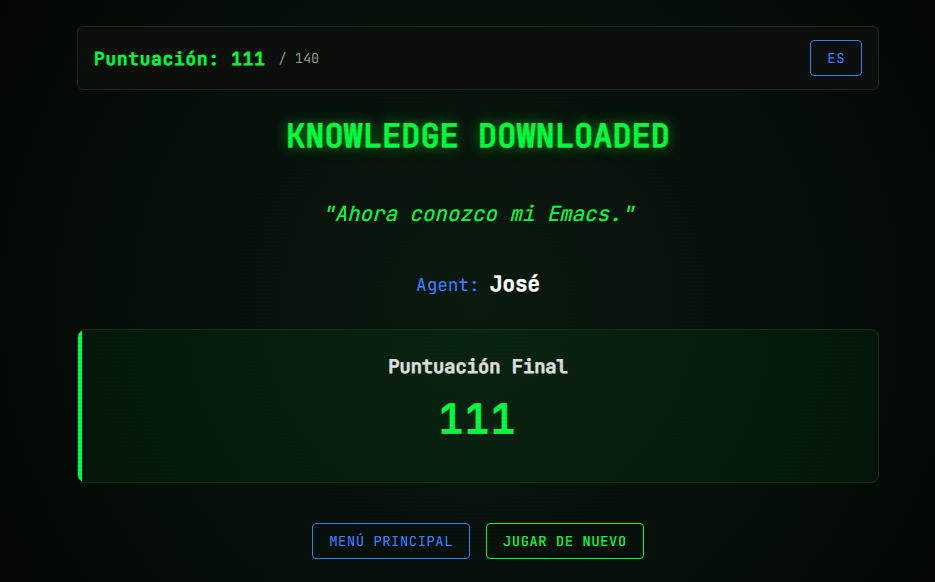
\includegraphics[width=.9\linewidth]{Fotos/IntentoJuego1JJ.jpeg}
\end{center}
-Intento2
\begin{center}
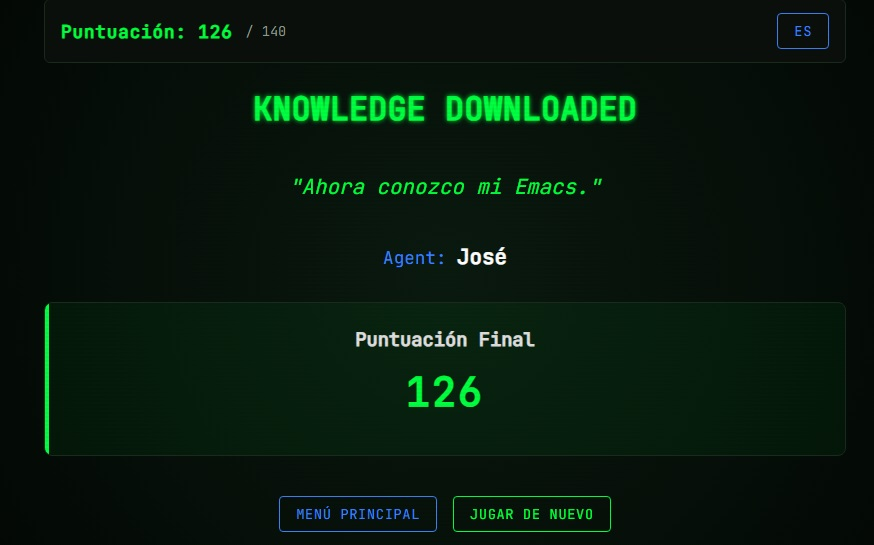
\includegraphics[width=.9\linewidth]{Fotos/IntentoJuego2JJ.jpeg}
\end{center}
-Intento3
\begin{center}
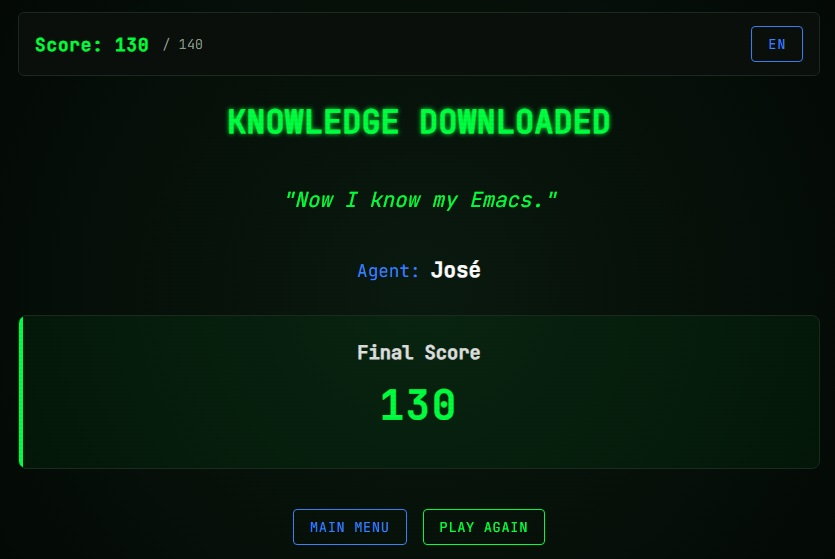
\includegraphics[width=.9\linewidth]{Fotos/IntentoJuego3JJ.jpeg}
\end{center}

Samuel Churaco: 
\begin{center}
\begin{tabular}{rr}
\hline
iteración & Puntaje\\[0pt]
\hline
1 & 110\\[0pt]
2 & 120\\[0pt]
3 & 140\\[0pt]
\hline
\end{tabular}
\end{center}

-Intento 1
  \begin{center}
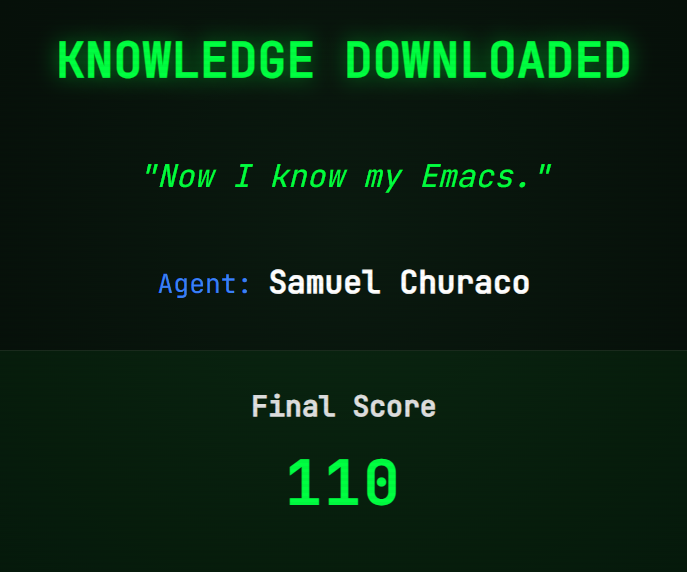
\includegraphics[width=.9\linewidth]{Fotos/IntentS1.png}
\end{center}
-intento 2
  \begin{center}
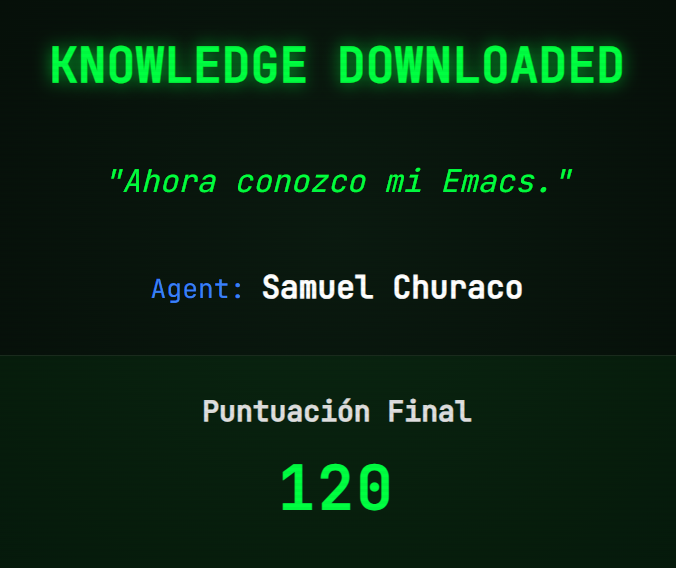
\includegraphics[width=.9\linewidth]{Fotos/IntentS2.png}
\end{center}
-Intento 3
  \begin{center}
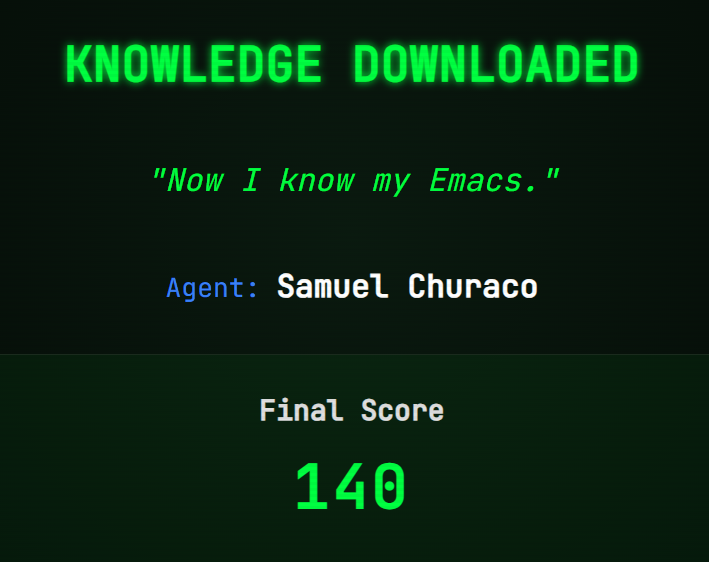
\includegraphics[width=.9\linewidth]{Fotos/IntentS3.png}
\end{center}

\subsection{Usando Emacs para tener Ayuda sobre Emacs}
\label{sec:org1be95ea}
¿Qué comandos le resultan más fáciles de usar y cuáles le son más
extraños? Identifique 4 comandos que le sean fáciles y 4 que le
resulten complicados. Revise qué dice la ayuda de Emacs sobre cada
comando y escriba en sus palabras el para qué sirve.

Para consultar lo que hace un comando ejecute:
\begin{enumerate}
\item \texttt{C-h k}
\item Emacs le preguntara cuál es la combinación de la que requiere
ayuda. Presione las teclas del comando. Por ejemplo, \texttt{C-x C-f}
\item Emacs abrirá un nuevo buffer con la descripción del comando.
\item Cambie al buffer de la ayuda con \texttt{C-x o}
\item Seleccione el primer parrafo de ayuda ubicando el cursor al inicio
del parrafo y activando la marcación de texto con
\texttt{C-SPC}. Seleccione avanzando por palabras \texttt{M-f} o directamente
toda la linea \texttt{C-e}
\item Una vez seleccionado, copie el texto con \texttt{M-w}.
\item Regrese al buffer anterior con \texttt{C-x o}.
\item Pegue el texto en <Pegar lo que dice el\ldots{}> con \texttt{C-y}
\end{enumerate}

\textbf{\textbf{Comandos Fáciles}}
\begin{enumerate}
\item \textbf{\textbf{Leonardo Rodriguez:}} <C-x C-f>. <Edit file FILENAME.
\end{enumerate}
Switch to a buffer visiting file FILENAME, creating one if none
already exists.
Interactively, the default if you just type RET is the current directory,
but the visited file name is available through the minibuffer history:
type M-n to pull it into the minibuffer.>
>
\begin{enumerate}
\item **Samuel Churaco**<C-x - o >. <
\end{enumerate}
Select another window in cyclic ordering of windows.
COUNT specifies the number of windows to skip, starting with the
selected window, before making the selection.  If COUNT is
positive, skip COUNT windows forwards.  If COUNT is negative,
skip -COUNT windows backwards.  COUNT zero means do not skip any
window, so select the selected window.  In an interactive call,
COUNT is the numeric prefix argument.  Return nil.
 >
\begin{enumerate}
\item \textbf{\textbf{José Jácome:}} <C-x u>. <C-x u runs the command undo (found in global-map), which is an
\end{enumerate}
interactive native-compiled Lisp function in ‘simple.el’.
It is bound to C-\_, <undo>, C-/ and C-x u.
It can also be invoked from the menu: Edit → Undo
(undo \&optional ARG)
Undo some previous changes.
Repeat this command to undo more changes>

\begin{enumerate}
\item <C-x C-s> <It can also be invoked from the menu: File → Save
\end{enumerate}

(save-buffer \&optional ARG)

Save current buffer in visited file if modified.
Variations are described below.>
\textbf{\textbf{Comandos Difíciles}}
\begin{enumerate}
\item \textbf{\textbf{Leonardo Rodriguez:}} <C-s>. <It is bound to C-s.
\end{enumerate}
It can also be invoked from the menu: Edit → Incremental Search →
Forward String\ldots{}>
\begin{enumerate}
\item \textbf{\textbf{Samuel Churaco:}} <C-x -d>. <"Edit" directory DIRNAME--delete, rename, print, etc. some files in it.
\end{enumerate}
Optional second argument SWITCHES specifies the options to be used
when invoking ‘insert-directory-program’, usually ‘ls’, which produces
the listing of the directory files and their attributes.
Interactively, a prefix argument will cause the command to prompt
for SWITCHES.
>
\begin{enumerate}
\item \textbf{\textbf{José Jácome:}} <C-M-v>. <C-M-v runs the command scroll-other-window (found in global-map),
\end{enumerate}
which is an interactive native-compiled Lisp function in ‘window.el’.
It is bound to M-<next>, C-M-v and ESC <next> .>
\begin{enumerate}
\item <C-x b> <Set the mark where point is, and activate it; or jump to the mark.
\end{enumerate}
Setting the mark also alters the region, which is the text
between point and mark; this is the closest equivalent in
Emacs to what some editors call the "selection".>
\section{Equipo de Trabajo}
\label{sec:org4fc780e}
Complete la información de los integrantes de grupo e indique el líder
de grupo.

\begin{center}
\begin{tabular}{lll}
\hline
Nombre & email & Rol\\[0pt]
\hline
Samuel Churaco & samuel.churaco@epn.edu.ec & Líder\\[0pt]
José Jácome & jose.jacome04@epn.edu.ec & Colaborador\\[0pt]
Leonardo Rodriguez & leonardo.rodriguez01@epn.edu.ec & Colaborador\\[0pt]
\hline
\end{tabular}
\end{center}

\section{Verificación de Entregables [100\%]:}
\label{sec:orga497dd9}
Ejecute \texttt{C-c C-c} sobre los ítems de tarea según se hayan cumplido o
no. Si un ítem no pudo realizarse apunte en la siguiente sección las
razones al respecto.
\begin{itemize}
\item[{$\boxtimes$}] Verificación de configuración de entorno WSL y paquetes del curso.
\item[{$\boxtimes$}] Tutorial de Comandos Emacs realizado.
\item[{$\boxtimes$}] Captura de Imágenes y puntajes de Emacs Trainer App.
\item[{$\boxtimes$}] Usando Emacs para tener ayuda sobre Emacs
\item[{$\boxtimes$}] Verifique que estén los nombres de los integrantes del equipo e
identificado el líder.
\item[{$\boxtimes$}] Revisión de ortografía con \texttt{ispell} en el buffer
\item[{$\boxtimes$}] Generación de Archivo PDF \texttt{M-x org-latex-export-to-pdf}
\end{itemize}
\subsection{Problemas con la Tarea:}
\label{sec:org9bea53e}
\begin{itemize}
\item Tarea \(X_1\) no pudo completarse debido a
\item Tarea \(X_2\) no pudo completarse debido a
\end{itemize}
\end{document}
